\documentclass[serif]{beamer}
\usepackage[orientation=landscape,size=a0,scale=1.4]{beamerposter}
\usepackage{hyperref} %enable hyperlink for urls
\usepackage[font=scriptsize,justification=justified]{caption}

\newcommand\apj{ApJ}
\newcommand\prd{PRD}
\newcommand\nat{Nature}

\usepackage{ragged2e}

\usepackage{amsmath,amssymb,mathtools}

\usepackage{multicol}

% Replacement palatino fonts
% Would set osf here, but see below
% largesc -> make the small-caps an iota larger (so they match the roman miniscules)
% tighter -> adopt pxfonts spacings (to exploit the better kerning) instead of pagella
% upint -> upright integrals (use much less hspace)
% smallerops -> make the sum/product operators more squat and square
% slantedGreek -> loads italic captical math greeks, to match italic capital math latin
% varbb -> use a less ugly though less conventional blackboard bold DISABLED (see below)
\usepackage[largesc,tighter]{newpxtext}
% Switch the Palatino numbers to the gorgeous `old style' ones. This must be done here
% not as a package option or Babel gets sad. Do it *Before* newpxmath to get osf numbers in maths.
\useosf
\usepackage[upint,smallerops,slantedGreek]{newpxmath}
% Better typewriter font (mono makes it a proper TT font -- currently unsupported though!); 0.9 scales it to the px sizes.
\usepackage[scaled=0.9]{inconsolata}
% Pretty mathcal font, scaled down v. slightly (+ load a decent mathscr font, switch the slightly better looking esstix frakturs and the inordinately better txof bbold)
\usepackage[cal=rsfso,calscaled=.96,scr=rsfs,scrscaled=.96,frak=esstix,frakscaled=.98,bb=txof,bbscaled=1.05]{mathalfa}
\usepackage{xcolor,mdframed}

\renewcommand\rmdefault{pplx}
\renewcommand\mathfamilydefault{cmr}

\setbeamertemplate{bibliography item}{\insertbiblabel}

\setbeamertemplate{caption}[numbered]
%\setbeamertemplate{enumerate}[circle]
\setbeamertemplate{items}[circle]

\definecolor{ETH1}{RGB}{31,64,122}
\definecolor{ETH3}{RGB}{0,105,180}
\definecolor{ETH6}{RGB}{111,111,110}
\definecolor{ETH8}{RGB}{0,122,146}
\definecolor{ETH10}{RGB}{130,190,30}
\definecolor{tlg}{RGB}{230,230,230}

%%%%%%%%%%%%%%%%%%%%%%%%%%%%%%%%%%%%%%%%%%%%%%%%%%%%%%%%%%%%%%%%%%%%%%%%%%%%%%%%%%%%%%%%%%%%%%%%%%%%
%It seems many of the following entries do not control any visible Behaviour. All such entries are
%set to red, so that they are easy to spot if they ever become visible

\setbeamercolor{headline}{fg=red,bg=white} % This is the recommended color for Specialist community usage: change to ETH1 for general communication
\setbeamercolor{footline}{fg=red, bg=red}
\setbeamerfont{footline}{size=\large,series=\bf}
\setbeamercolor{separation line}{bg=ETH6}
\setbeamercolor{title in headline}{fg=ETH3}
\setbeamercolor{author in headline}{fg=ETH3}
\setbeamercolor{institute in headline}{fg=ETH3}

\setbeamercolor{framesubtitle}{fg=red, bg=ta2gray}
\setbeamercolor{author in head/foot}{fg=ETH3, bg=white}
\setbeamercolor{title in head/foot}{fg=red, bg=red}

\setbeamercolor*{normal text}{fg=ETH6, bg=white}
\setbeamercolor*{block body}{fg=black, bg=white}
\setbeamercolor*{block title}{fg=white,bg=ETH3}
\setbeamerfont{block title}{size=\large,series=\bf}
\setbeamercolor{upper separation line head}{fg=red}

\setbeamercolor*{example body}{fg=red,bg=red}
\setbeamercolor*{example text}{fg=red,bg=red}
\setbeamercolor*{example title}{bg=red,fg=red}

\setbeamercolor{alerted text}{fg=red}
\setbeamercolor{structure}{fg=black}

%\setbeamercolor{itemize item}{fg=ETH3}
%\setbeamertemplate{items}[square]
%\setbeamertemplate{itemize items}{\color{ETH3}$\blacktriangleright$}
\setbeamertemplate{navigation symbols}{}  % no navigation on a poster

\setbeamertemplate{headline}{
	\leavevmode
	\begin{beamercolorbox}[wd=\paperwidth]{headline}
		\vspace{2ex}
		\begin{columns}[c]
			\begin{column}{.09\paperwidth}
			\end{column}
			\begin{column}{.675\paperwidth}
				\raggedleft
				\usebeamercolor{title in headline}{\color{fg}\textbf{\LARGE{\inserttitle}}\\[1ex]}
				\usebeamercolor{author in headline}{\color{fg}\large{\insertauthor}\\[1ex]}
				\usebeamercolor{institute in headline}{\color{fg}\small{\insertinstitute}}
			\end{column}
			\begin{column}{.25\paperwidth}
				\begin{center}
					
\includegraphics[width=.8\textwidth, height=.3\textwidth, keepaspectratio]{Images/RIT2}
				\end{center}
			\end{column}
			\begin{column}{.03\paperwidth}
			\end{column}
		\end{columns}
		\vspace{2ex}
	\end{beamercolorbox}

 	% \begin{beamercolorbox}[wd=\paperwidth]{lower separation line head}
	% 	\rule{0pt}{2pt}
	% \end{beamercolorbox}
	\vskip-2cm
	}

%%%%%%%%%%%%%%%%%%%%%%%%%%%%%%%%%%%%%%%%%%%%%%%%%%%%%%%%%%%%%%%%%%%%%%%%%%%%%%%%%%%%%%%%%%%%%%%%%%%%
\setbeamertemplate{footline}{
	\begin{beamercolorbox}[wd=\paperwidth]{upper separation line foot}
		\rule{0pt}{2pt}
	\end{beamercolorbox}
	\leavevmode%
	\begin{beamercolorbox}[ht=4ex,leftskip=1cm,rightskip=1cm]{author in head/foot}%
        Aasim Z Jan (RIT)
		\hfill
		September 15th, 2020
        \hfill
        \href{https://dcc.ligo.org/LIGO-G2001500}{LIGO-G2001500}
		\hfill
		Aasim.jan@ligo.org
		\vskip1ex
	\end{beamercolorbox}
	\vskip0pt%
	\begin{beamercolorbox}[wd=\paperwidth]{lower separation line foot}
		\rule{0pt}{2pt}
	\end{beamercolorbox}
	}


\input{paper_submodules/O2RandPPaper/rates_macros.tex}
\input{paper_submodules/O2RandPPaper/SDDR_macros.tex}
\input{paper_submodules/O2RandPPaper/pe_macros.tex}

%% Units and common defs
\def\Msol{\ensuremath{\mathit{M_\odot}}}
\newcommand\unit[1]{{\rm #1}}

% Parameters
\def\mchirp{\ensuremath{\mathcal{M}_c}{}}
\def\chieff{\ensuremath{\chi_{\textrm{eff}}}{}}
\def\chip{\ensuremath{\chi_p}{}}

\def\mmax{\ensuremath{m_{\textrm{max}}}{}}
\def\mmin{\ensuremath{m_{\textrm{min}}}{}}
\def\mtotmax{\ensuremath{M_{\textrm{max}}}{}}

\def\rater{\ensuremath{\mathcal{R}}{}}
\def\Vc{\ensuremath{V_c}{}}
\def\VT{\ensuremath{\langle VT \rangle}{}}

% commands - \SI{number}{units}  or \si{units}
\newcommand{\SI}[2]{\ensuremath{#1\,{\rm #2}}{}}
\newcommand{\si}[1]{\ensuremath{\rm #1}{}}
\newcommand{\intrv}[3]{\ensuremath{#1_{-#2}^{+#3}}{}}

\def\invstvol{Gpc$^{-3}$ yr$^{-1}$}



\title{
%
  Assessing and marginalizing over CBC waveform systematics with RIFT
%
}
\author{
%
Aasim Z Jan, Anjali B Yelikar, Jacob Lange and Richard O'Shaughnessy                      %
%
}
\institute{}
\date{September 15th, 2020}


\begin{document}
\begin{frame}{}

\begin{columns}

\begin{column}[T]{.3\textwidth}

\begin{block}{Introduction}
 % The LIGO and Virgo instruments have detected ten black
  %hole binaries in the first two observing runs \cite{o2catalog}.
 Parameter estimation of Gravitational Wave signals is a key part of Gravitational Wave Astronomy and Astrophysics. Unbiased and reliable parameter estimation help achieve a higher precision for tests of General Relativity \cite{Shaik:2019dym}. However, waveforms used to perform parameter estimation produce systematic biases \cite{Veitch:2014wba}. The goal here is to reassess and mitigate these biases using RIFT. % \cite{Purrer:2019jcp}.
%  \begin{center}
 %  \begin{columns}
   %   \begin{column}[c]{0.45\textwidth}
      %  \centering
        %\includegraphics[width=\textwidth]{paper_submodules/cbc-catalog/figures/m1_m2_90pc.pdf}
      %\end{column}
      %~
      %begin{column}[c]{0.45\textwidth}
        %\centering
        %\includegraphics[width=\textwidth]{paper_submodules/cbc-catalog/figures/q_chieff_low_high}
      %\end{column}
    %\end{columns}
    %\includegraphics[width=\textwidth]{paper_submodules/cbc-catalog/figures/event_legend_all_ncol6}
    %\vspace{-6.5em}

  %\end{center}

  %emph{
    %\footnotesize
    %Figure: Mass and spin parameter estimates on the ten detected BBH's
    %and one BNS.

    %The BNS is not considered in this analysis.
 % }

  %\vspace{1em}

  %e use these observations to place constraints on the astrophysical
  %distribution of black hole binary masses, spins, and redshifts \cite{LIGO-O2-Rates}.


\end{block}

\vspace{1em}

\begin{block}{RIFT}
%\emph {Stands for}:
\textbf{R}apid parameter inference on Gravitational Wave sources via \textbf{I}terative \textbf{F}i\textbf{T}ing
is a two-stage iterative process to interpret Gravitational Wave observations via comparison to predicted Gravitational Wave signals \cite{Lange2018RapidAA}.
\vspace{1em}

\textbf{\emph{Stage 1}}: Compute marginal likelihood values for each point in parameter space ($\lambda_\alpha$) from a ``proposed grid''.
\vspace{0.1em}

\textbf{\emph{Stage 2}}: Generate an approximation to likelihood values (${\cal L}(\lambda)$) based on RIFT's
accumulated archived knowledge of marginal likelihood evaluations 
$(\lambda_\alpha,{\cal L}_\alpha)$ and from that approximation generate the (detector-frame) posterior distribution.




\begin{center}
	\begin{figure}
	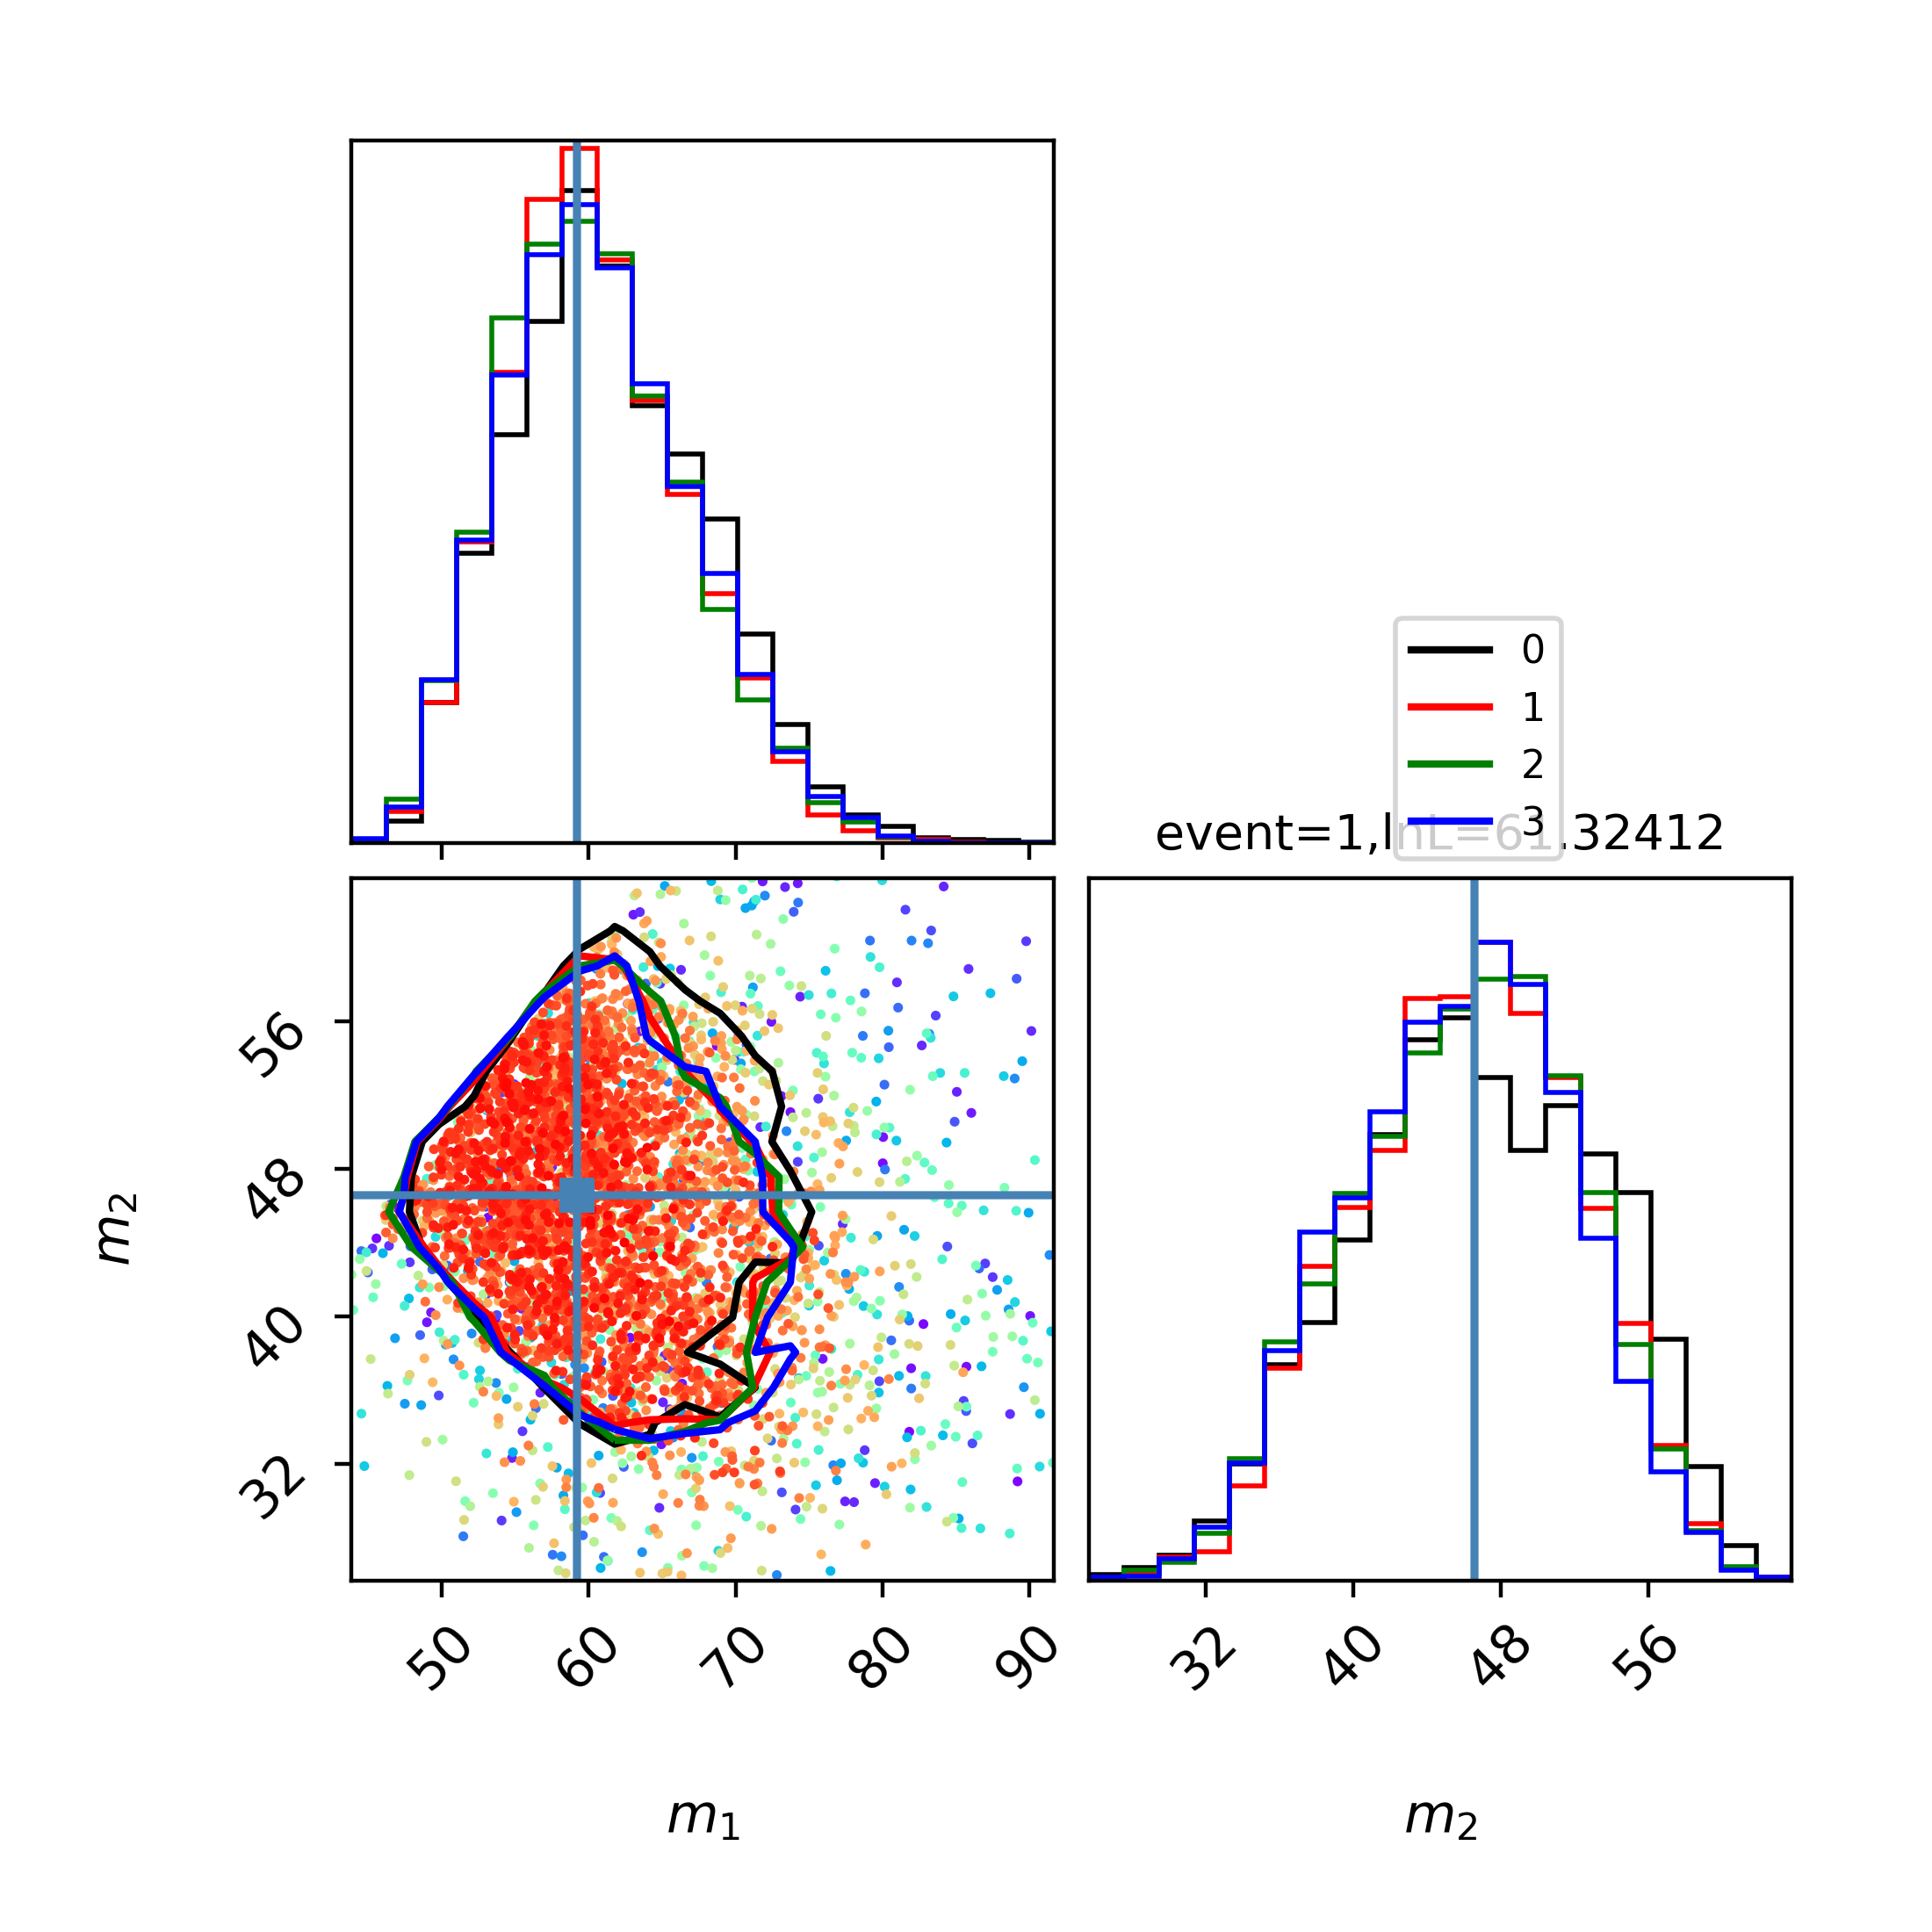
\includegraphics[scale=1.0]{Images/corner_m1_m2}
	\vspace{-1.0em}
	
	\small{\emph{\textbf{Figure 1:} Likelihood and posteriors obtained using RIFT}}
	\end{figure}

\end{center}
%\vspace{-1.25em}


\small{
This figure shows inferred posterior parameter distributions for a non-precessing Binary Blackhole source using RIFT. The blue crosshairs indicate true parameter values and contours in two dimensional plots (bottom left) indicate the 90\% credible region as estimated by each iteration. The colors correspond to different iterations. 

}
\end{block}



\end{column}
~
\begin{column}[T]{0.35\textwidth}

\begin{block}{Probability-Probability plots ($P$--$P$ plots)} 
\textbf{Basic Idea}: $x$--axis shows the probability contained in a credible interval and $y$--axis shows the fraction of true values which lay inside that interval. They are used to quantify two or more data sets. When injection and recovery is performed using the same model, we expect the $P$--$P$ plot to be a line of form $y=x$.  However, if recovery is performed using a different waveform model, the $P$--$P$ plot strays more from the expected $y=x$ behavior.



\begin{center}
  \vspace{-1.450em}
  \begin{center}

    \begin{columns}
      \begin{column}{0.45\textwidth}
      \begin{figure}
        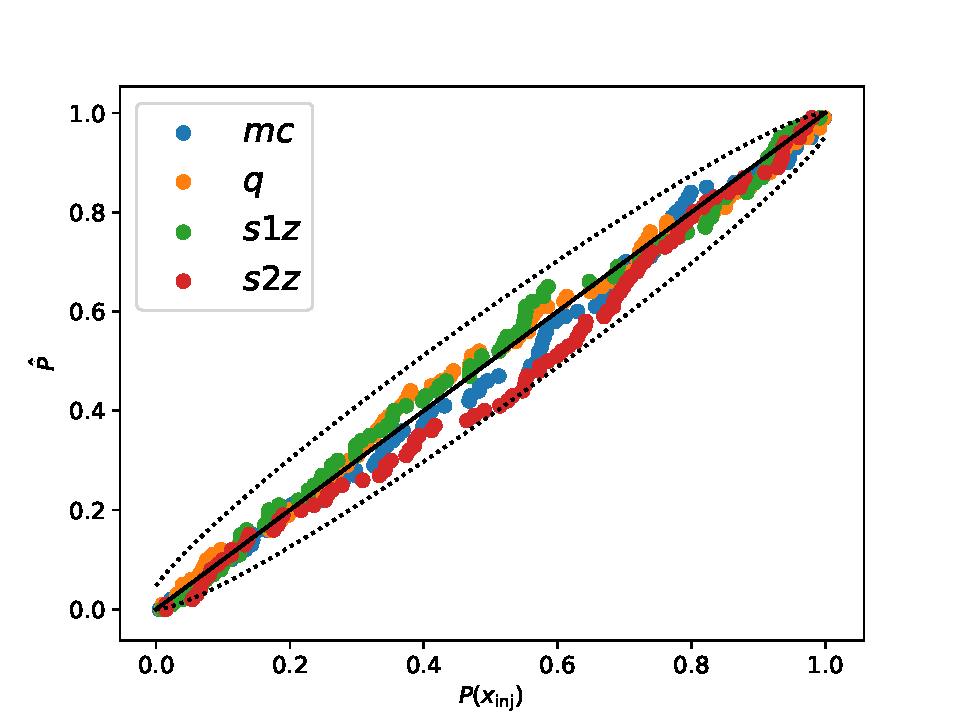
\includegraphics[scale=1.3]{Images/pp_plot_SEOB}
        \small{\emph{Injection: SEOBNRv$4$ \vspace{0.1em} 
        
        Recovery: SEOBNRv$4$}}
        \end{figure}
      \end{column}
       
      \begin{column}{0.45\textwidth}
      \begin{figure}
       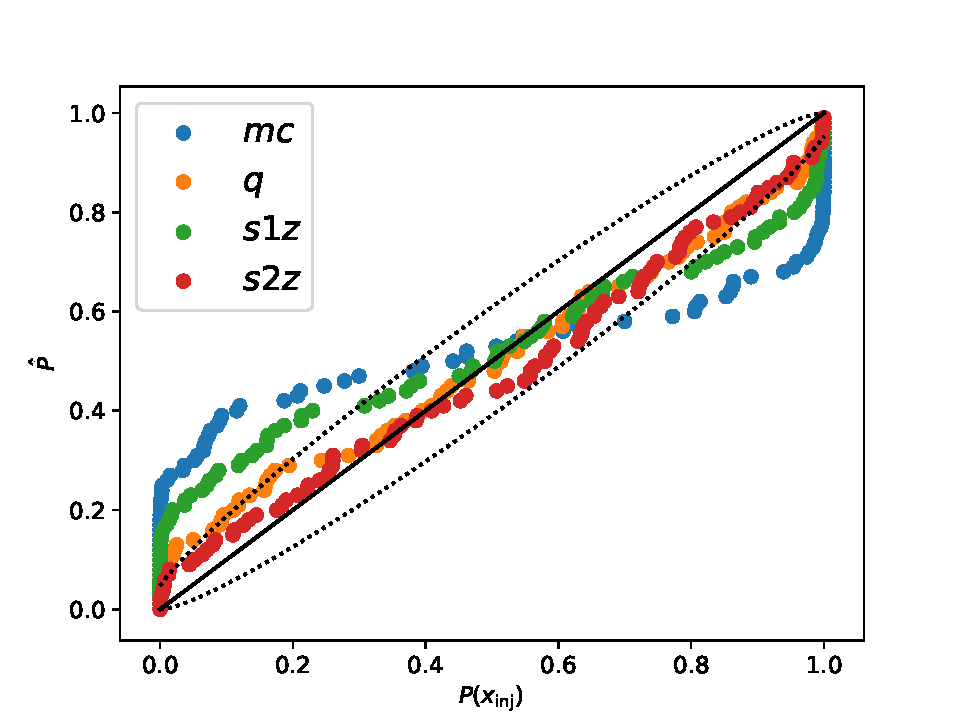
\includegraphics[scale=1.3]{Images/pp_plot_IMRD}
       \small{\emph{Injection: SEOBNRv$4$ \vspace{0.1em} 	
       
       Recovery: IMRPhenomD}}
       \end{figure}
      \end{column}
    \end{columns}
    \vspace{0.4em}
 \emph{ \small{\textbf{Figure 2:} $P$--$P$ plots for $100$ non-precessing Binary Black Hole (BBH) events.}}
   \end{center}



%\caption{\small {We generated $100$ events using SEOBNRv$4$ and recovered them using SEOBNRv$4$, and as hoped we have a pp plot which looks like $y=x$, with some minor randomness around it}}
  \end{center}

  



\vspace{0.5em}

\normalsize{In our runs, the waveform model used for injection was known allowing us to run parameter inference and recover unbiased posterior samples. However, such is not usually the case paving the need for model marginalization.}
 

  \begin{center}
    \begin{columns}
      \begin{column}{0.45\textwidth}
        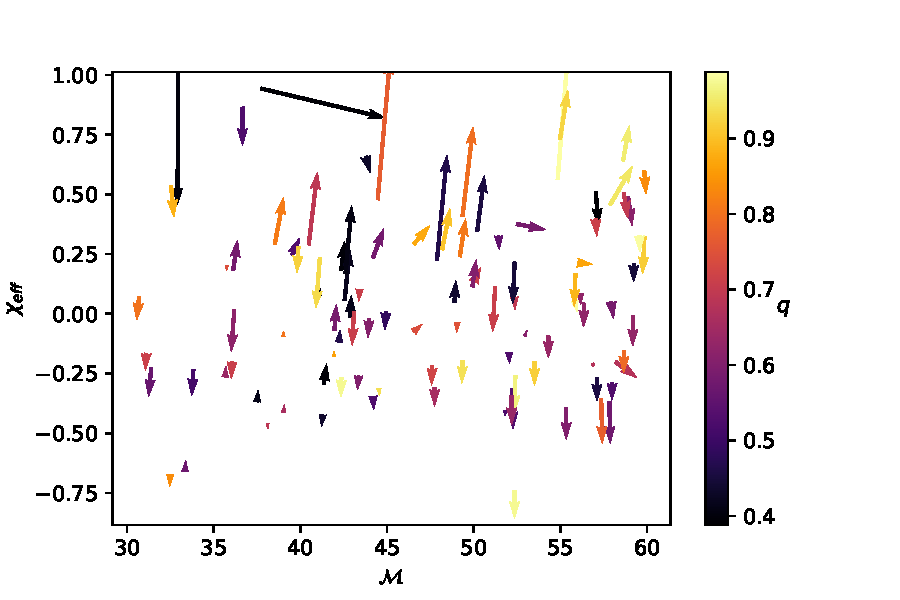
\includegraphics[scale=1.5]{Images/2D_mc_xi_vector_plot}
      \end{column}
       
      \begin{column}{0.45\textwidth}
       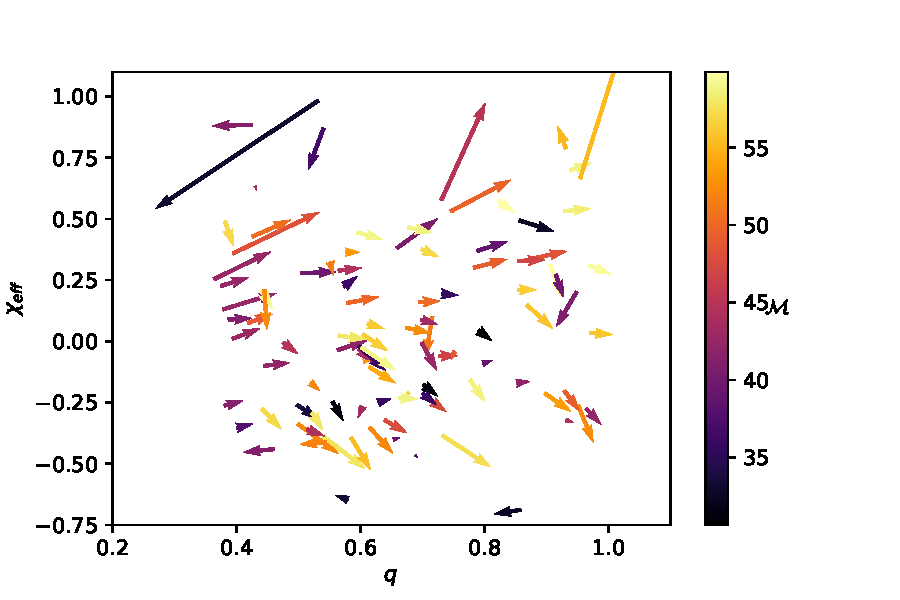
\includegraphics[scale=1.5]{Images/2D_q_xi_vector_plot}
      \end{column}
    \end{columns}
  \small{\emph{\textbf{Figure 3:} Systematic parameter biases}}
   \end{center}

%($x_{meanSEOBNRv4} - x_{meanIMRPhenomD})$/$(\sqrt{\sigma_(xSEOBNRv$4$)*\sigma_(xIMRPhenomD)}*SNR)$ 

 \small{The $x$ and $y$ axes on these vector plots are parameter values and length of the arrow denotes SNR-scaled offsets between parameters recovered by the two waveforms. The colormap is the value of the 3rd parameter($\mathcal{M}/q/\chi_{eff}$).}

\vspace{0.5em}

\normalsize{These plots were generated for zero-noise injections so we are seeing pure systematic differences between the two models. This plot shows that for a same event we will get different values from two different recovery models which might vary significantly.}




%\noindent \emph{Rate, mass distribution, and spin distribution correlated}: Joint inference! Strong correlation between mass
  %distribution features and merger rate.

\end{block}

%% \begin{block}{Parameter Constraints}
%%  key ideas:

%% - basic rate-shape correlation

%% - minimum mass not being informative.
%%       (Possibly show minimum mass down to 3 Msun as extra option?)
%% \end{block}

\vspace{1em}

%\begin{block}{Model Marginalization}






%\end{block}


\vfill
\end{column}
~
\begin{column}[T]{0.3\textwidth}


\begin{block}{Model Marginalization}
Based on Ashton and Khan \cite{Ashton:2019leq} description of marginalization between a discrete set of waveform models, we examine a waveform-marginalization technique. Operationally speaking, we construct model-averaged marginal likelihoods by the following procedure.

\vspace{-3.5em}
\begin{center}
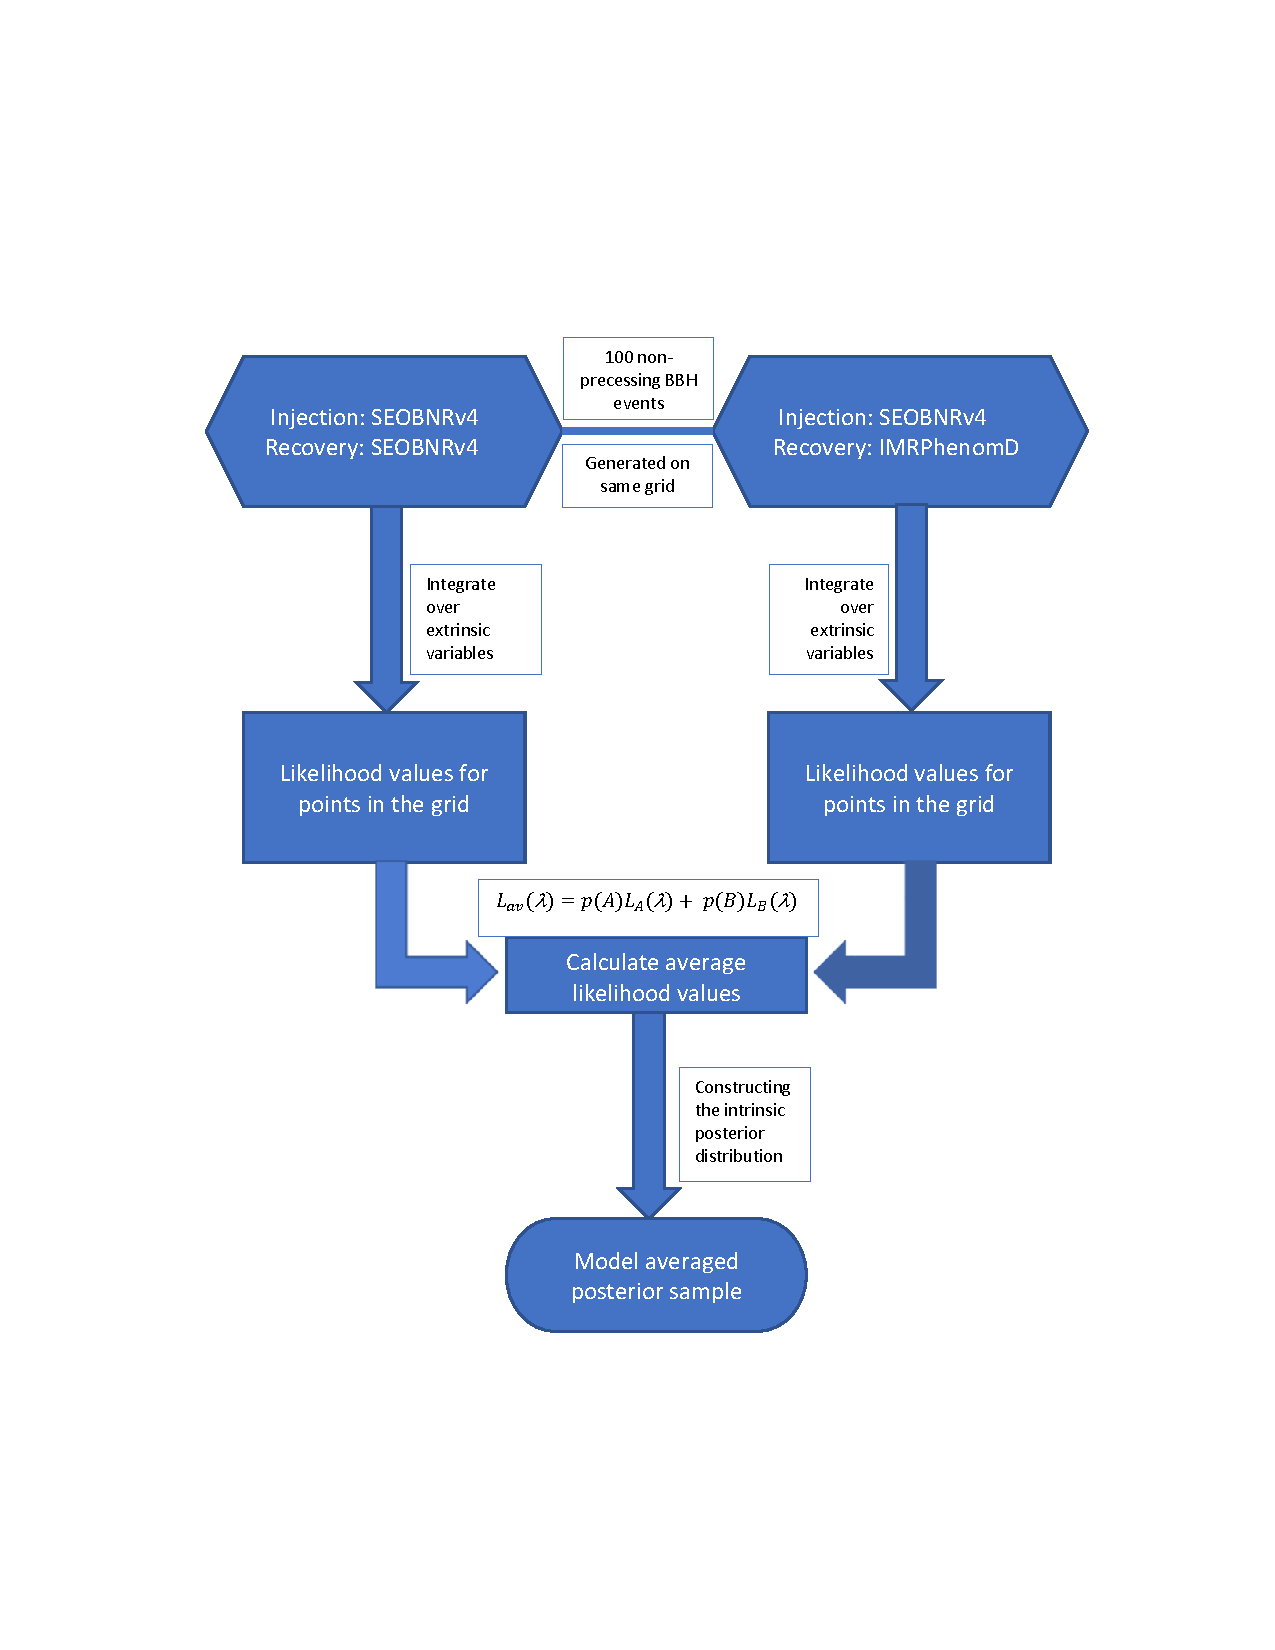
\includegraphics[width=330mm, height=300mm]{Images/Flow_chart}
\end{center}
\vspace{-4.4em}

\begin{center}
\small{\emph{\textbf{Figure 4:} Model marginalization flowchart}}
\end{center}

\vspace{-.5em}
\begin{center}
    \begin{columns}
      \begin{column}{0.45\textwidth}
        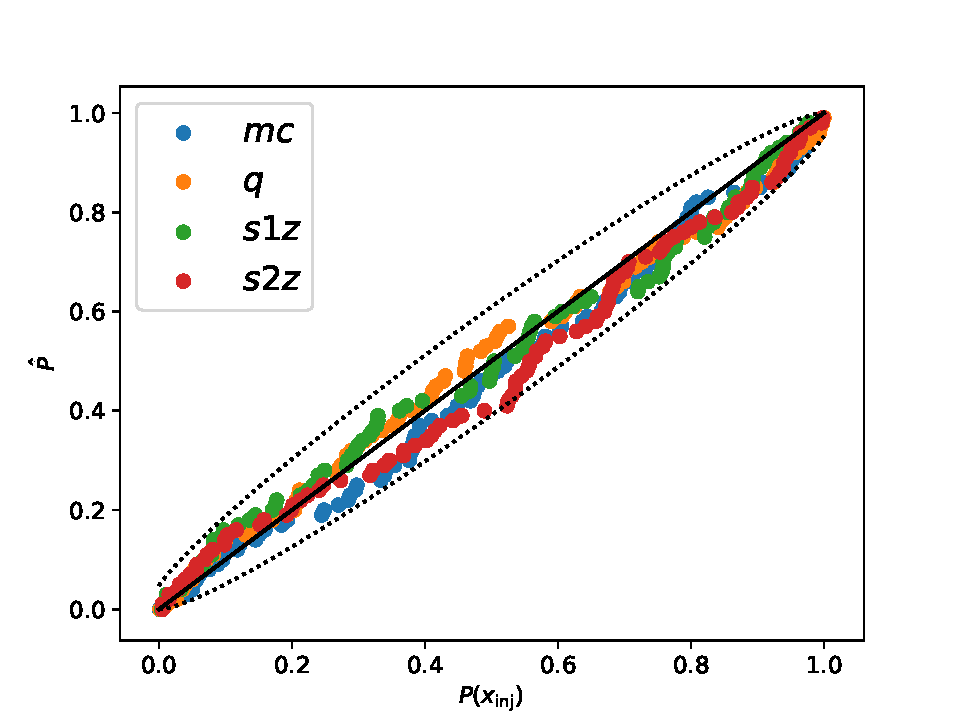
\includegraphics[scale=1.1]{Images/output_pp}
      \end{column}
       
      \begin{column}{0.45\textwidth}
       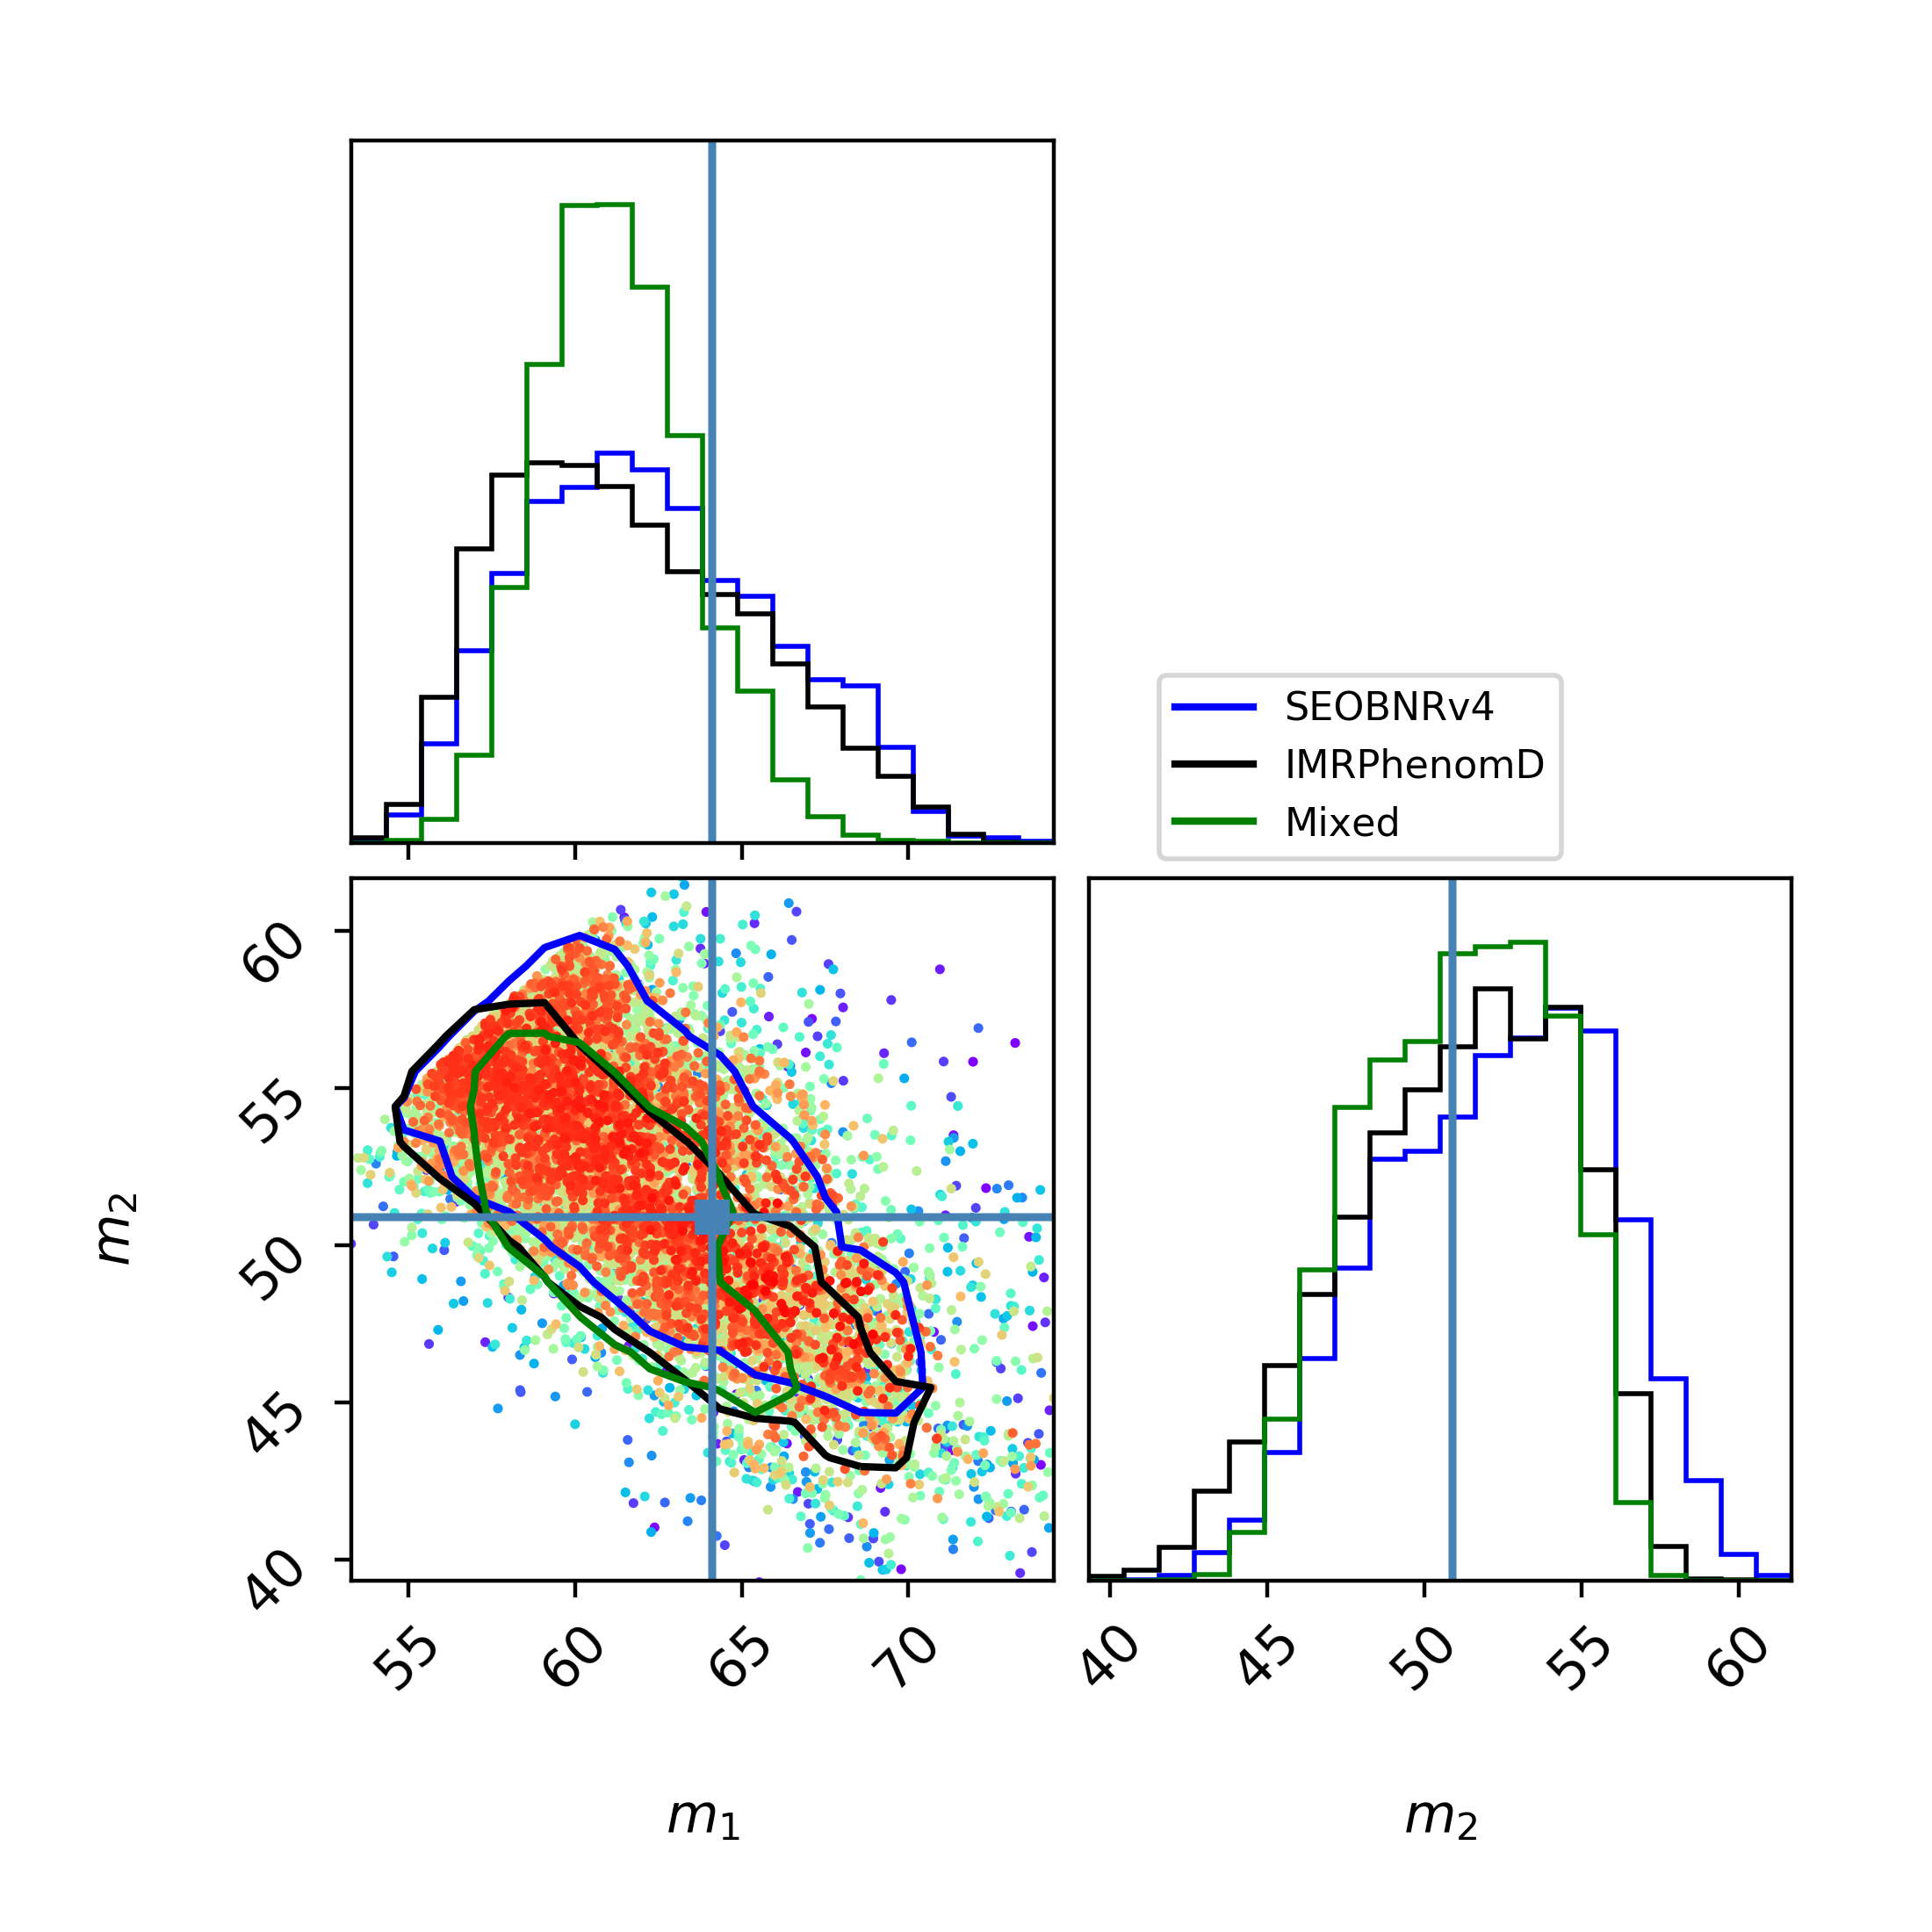
\includegraphics[scale=1.4]{Images/corner_m1_m2_event_65}
      \end{column}
    \end{columns}



\small{\emph{\textbf{Figure 5:} $P$--$P$ plot and posteriors for model marginalized runs}}
\vspace{0.1em}
\end{center}
\small{From the $P$--$P$ plot and the posteriors, it appears if we used model averaging we get results which are less biased.}


\vspace{-0.20em}




\end{block}

\vspace{0.5em}
\begin{block}{Conclusions}
In situations where injections aren't known, we can perform model marginalization and get better results than randomly choosing a waveform as recovery. And since this is based on RIFT, a very efficient parameter inference engine, our technique can include any available model, including very accurate but computationally costly estimates.
%\begin{itemize}
%\item Many Waveform templates out there, need a study that compares them to look for biases(if they exist)
% and deduce if they are due to noise statistics/systematics or underlying physics(phenomenological models, 
% NR simulations, NRhybrid waveforms). 
 %\item Statistical differences will arise due to noise fluctuations in the received signal, whereas systematic 
% differences will arise due to the inherent difference in the models/underlying physics.
 

%\end{itemize}


\end{block}

\end{column}

\end{columns}

\vspace{0.5em}

\begin{block}{References}
\vspace{-1em}
\begin{multicols}{2}
  {\tiny{
  \bibliographystyle{unsrt}
%    \bibliographystyle{abbrv}
    \bibliography{references.bib}  }}

\end{multicols}

% {\tiny
% %  \footnotesize
%   \bibliographystyle{unsrtnat}
%   \bibliography{paper_submodules/O2RandPPaper/references,poster.bib}
% }
\end{block}
\end{frame}
\end{document}

\small{
\item Construct a fiducial grid for waveform models A and B.
\item Use ILE to evaluate ${\cal L}_A(\lambda_k)$ and ${\cal L}_B(\lambda_k)$ on this grid.
\item Construct ${\cal L}_{av}(\lambda_k)$ as below.  
\begin{align}
{\cal L}_{av}(\lambda) = p(A) {\cal L}_A(\lambda) + p(B) {\cal L}_B(\lambda).
\end{align}
\item Use the combinations $(\lambda_k, {\cal L}_{av})$ with CIP, to construct a
model-averaged posterior distribution.
}






\begin{center}
    \begin{columns}
      \begin{column}{0.45\textwidth}
        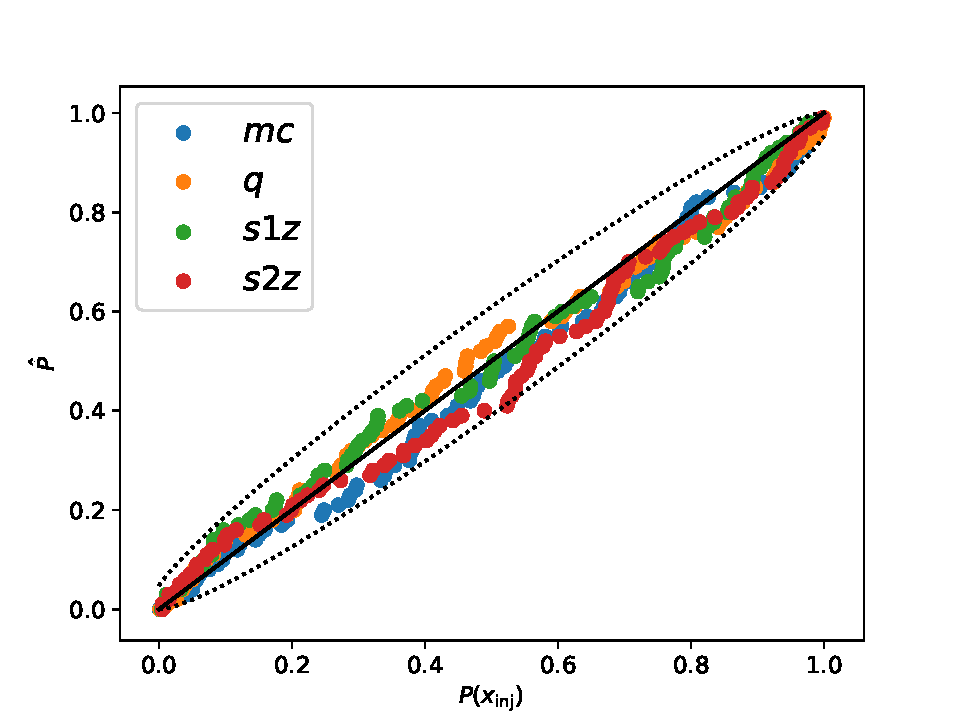
\includegraphics[scale=1.2]{Images/output_pp}
      \end{column}
       
      \begin{column}{0.45\textwidth}
       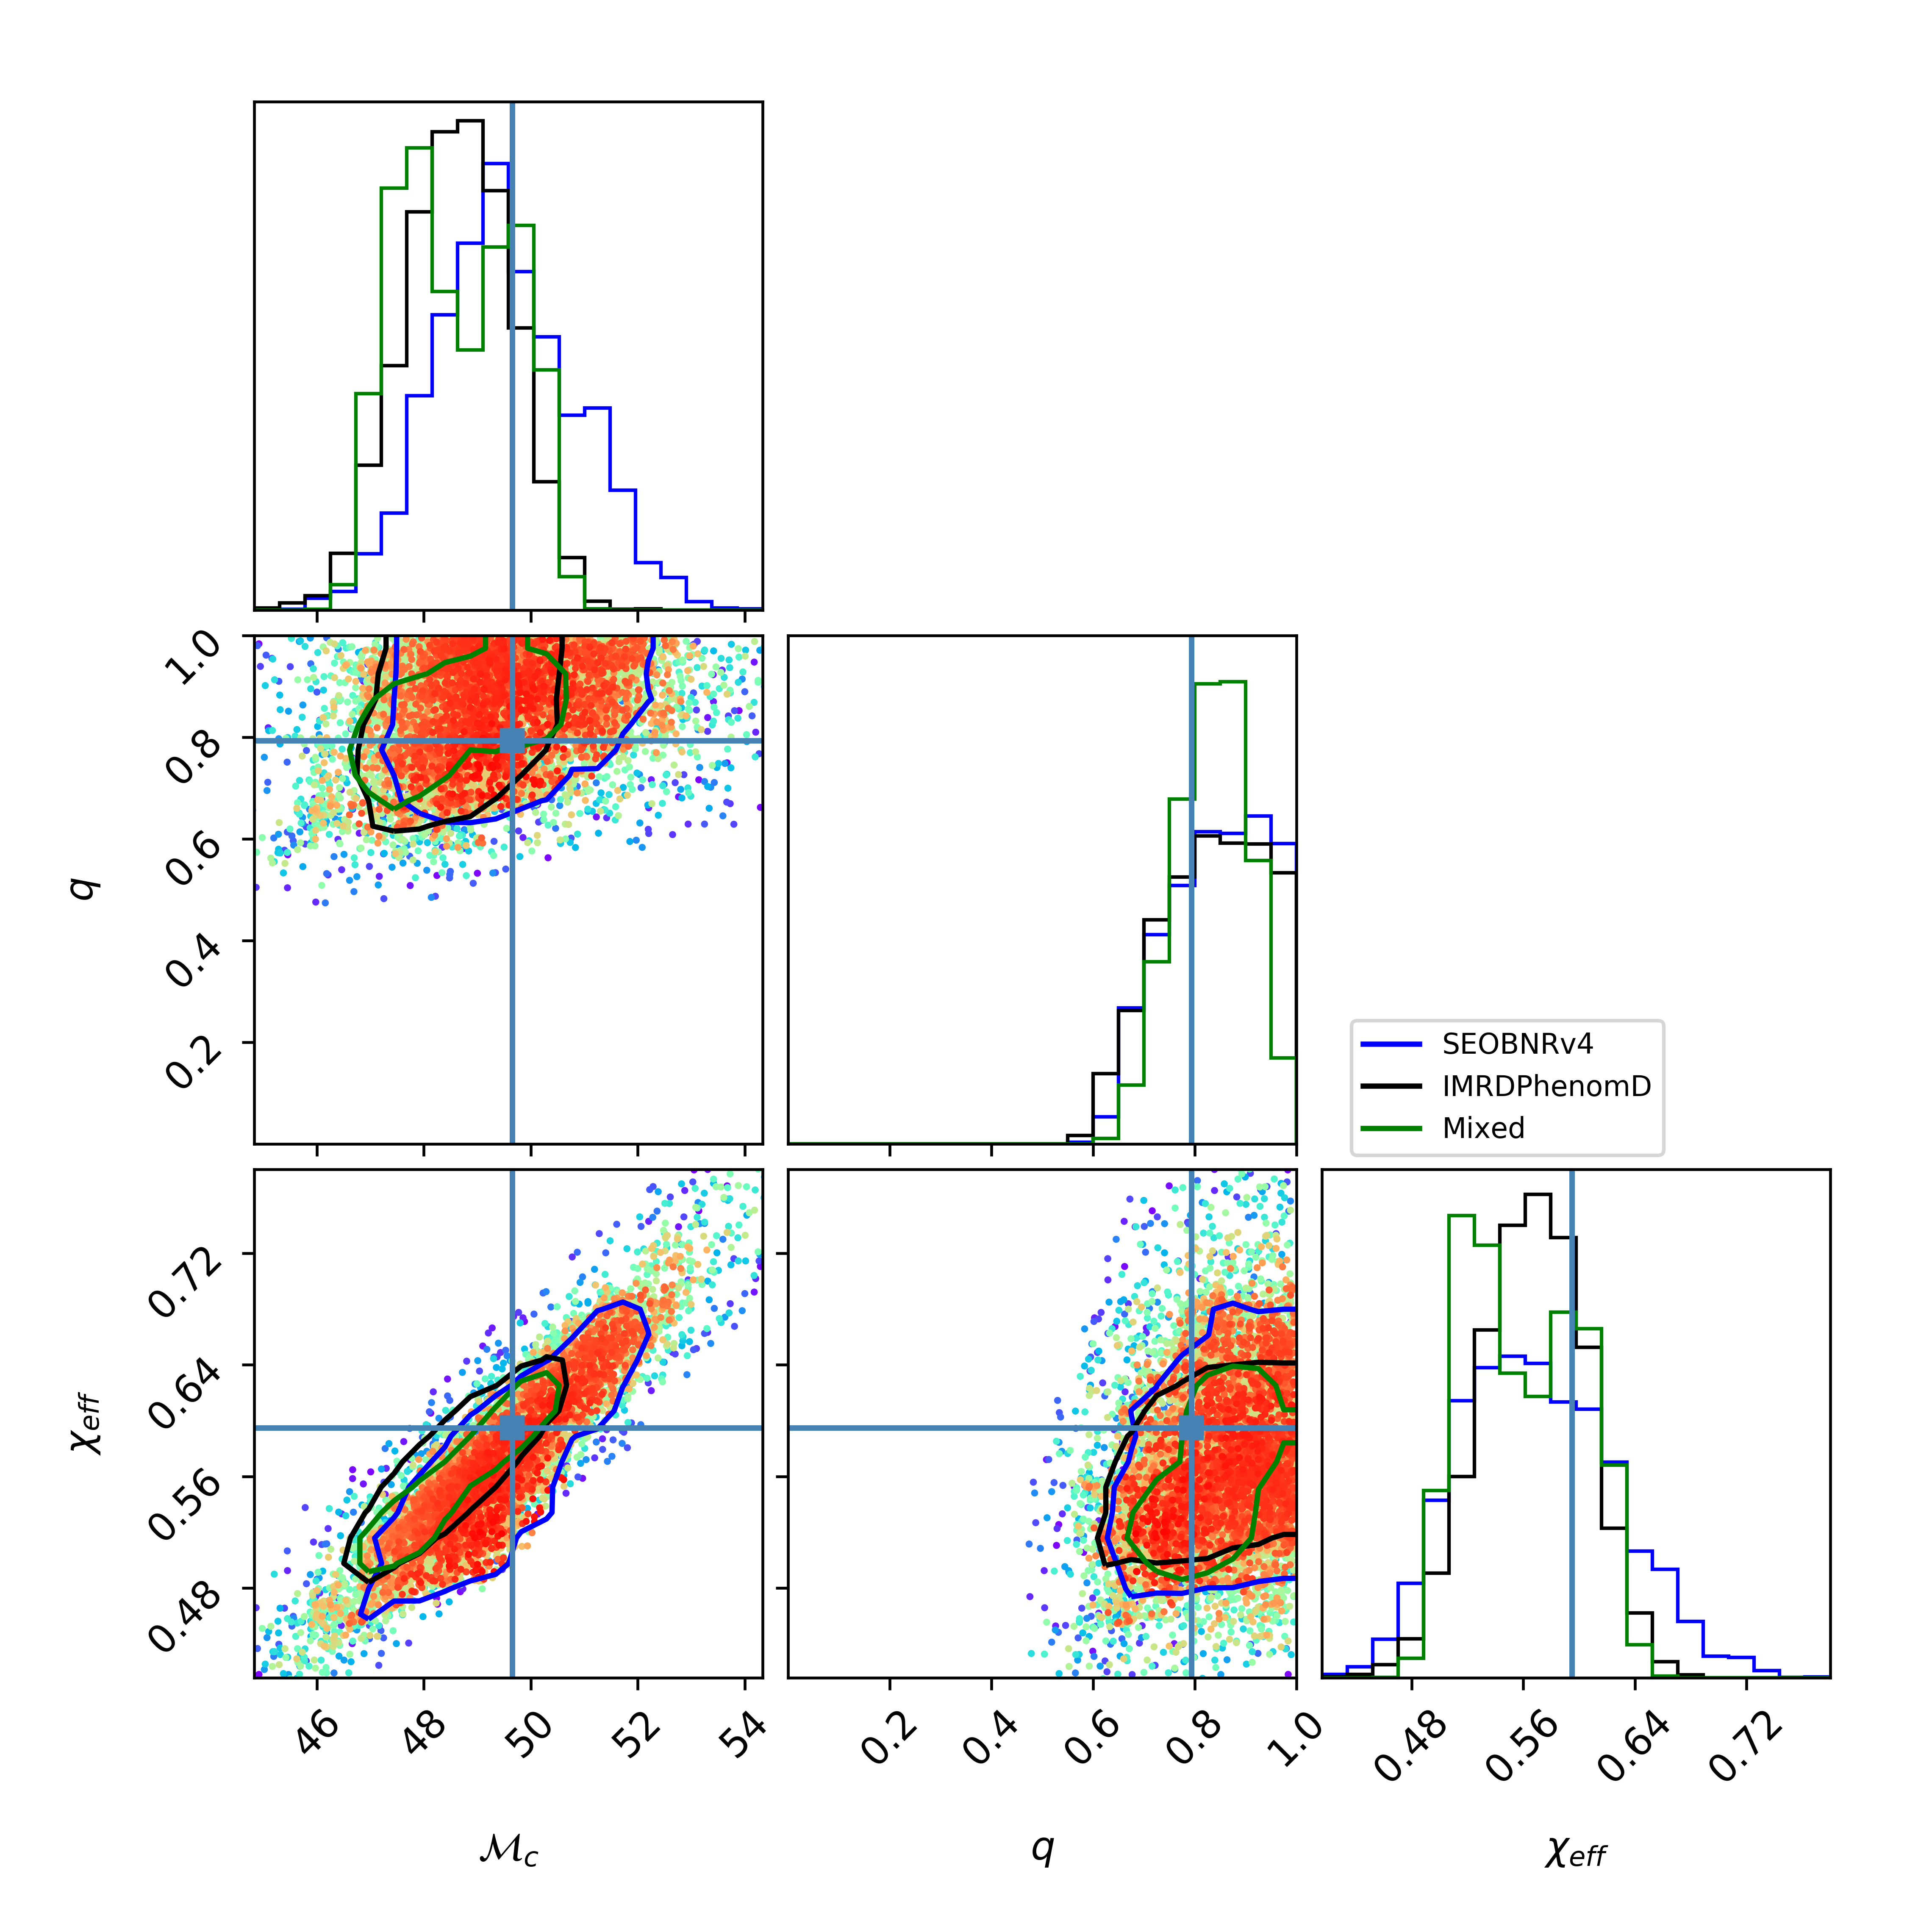
\includegraphics[scale=1.]{Images/corner_mc_q_xi_event_65}
      \end{column}
    \end{columns}
%   \end{center}


\small{The $P$--$P$ plot here was generated using model-averaged posterior distribution, and it can be observed that while the behavior is more random around $y=x$ when compared to just SEOBNRv$4$ recovery, it is much less random when compared to IMRPhenomD recovery. If the injection wasn't known, model averaging would give results which are less biased.}



